%保存为UTF-8编码格式
%用xelatex编译
 
\documentclass[UTF8,a4paper,11pt]{ctexart}
\usepackage[left=2.50cm, right=2.50cm, top=2.50cm, bottom=2.50cm]{geometry} %页边距
\CTEXsetup[format={\Large\bfseries}]{section} %设置章标题字号为Large,居左
%\CTEXsetup[number={\chinese{section}}]{section}
%\CTEXsetup[name={(,)}]{subsection}
%\CTEXsetup[number={\chinese{subsection}}]{subsection}
%\CTEXsetup[name={(,)}]{subsubsection}
%\CTEXsetup[number=\arabic{subsubsection}]{subsubsection}  %以上四行为各级标题样式设置,可根据需要做修改
 
%\linespread{1.5} %设置全文行间距
 
 
%\usepackage[english]{babel}
%\usepackage{float}     %放弃美学排版图表
\usepackage{fontspec}   %修改字体
\usepackage{amsmath, amsfonts, amssymb} % 数学公式相关宏包
\usepackage{color}      % color content
\usepackage{graphicx}   % 导入图片
\usepackage{subfigure}  % 并排子图
\usepackage{url}        % 超链接
\usepackage{bm}         % 加粗部分公式,比如\bm{aaa}aaa
\usepackage{multirow}
\usepackage{booktabs}
\usepackage{epstopdf}
\usepackage{epsfig}
\usepackage{longtable}  %长表格
\usepackage{supertabular}%跨页表格
\usepackage{algorithm}
\usepackage{algorithmic}
\usepackage{changepage}

\usepackage{listings}  %插入代码块
\usepackage{color}
\usepackage{xcolor}
\definecolor{dkgreen}{rgb}{0,0.6,0}
\definecolor{gray}{rgb}{0.5,0.5,0.5}
\definecolor{mauve}{rgb}{0.58,0,0.82}
\lstset{frame=tb,
     language=Java,
     aboveskip=3mm,
     belowskip=3mm,
     showstringspaces=false,
     columns=flexible,
     basicstyle = \ttfamily\small,
     numbers=none,
     numberstyle=\tiny\color{gray},
     keywordstyle=\color{blue},
     commentstyle=\color{dkgreen},
     stringstyle=\color{mauve},
     breaklines=true,
     breakatwhitespace=true,
     tabsize=3
}

\setcounter{secnumdepth}{4}
\setcounter{tocdepth}{4} 

%%%%%%%%%%%%%%%%%%%%%%%
% -- text font --
% compile using Xelatex
%%%%%%%%%%%%%%%%%%%%%%%
% -- 中文字体 --
%\setCJKmainfont{Microsoft YaHei}  % 微软雅黑
%\setCJKmainfont{YouYuan}  % 幼圆
%\setCJKmainfont{NSimSun}  % 新宋体
%\setCJKmainfont{KaiTi}    % 楷体
\setCJKmainfont{SimSun}   % 宋体
%\setCJKmainfont{SimHei}   % 黑体
 
% -- 英文字体 --
\setmainfont{Times New Roman}
%\setmainfont{DejaVu Sans}
%\setmainfont{Latin Modern Mono}
%\setmainfont{Consolas}
%
%
\renewcommand{\algorithmicrequire}{ \textbf{Input:}}     % use Input in the format of Algorithm
\renewcommand{\algorithmicensure}{ \textbf{Initialize:}} % use Initialize in the format of Algorithm
\renewcommand{\algorithmicreturn}{ \textbf{Output:}}     % use Output in the format of Algorithm
\renewcommand{\abstractname}{\textbf{\large {摘\quad 要}}} %更改摘要二字的样式
\newcommand{\xiaosi}{\fontsize{12pt}{\baselineskip}}     %\xiaosi代替设置12pt字号命令,不加\selectfont,行间距设置无效
\newcommand{\wuhao}{\fontsize{10.5pt}{10.5pt}\selectfont}
 
\usepackage{fancyhdr} %设置全文页眉、页脚的格式
\pagestyle{fancy}
\lhead{}           %页眉左边设为空
\chead{}           %页眉中间
\rhead{}           %页眉右边
%\rhead{\includegraphics[width=1.2cm]{1.eps}}  %页眉右侧放置logo
\lfoot{}          %页脚左边
\cfoot{\thepage}  %页脚中间
\rfoot{}          %页脚右边
 
 
\usepackage{hyperref} %bookmarks
\hypersetup{colorlinks, bookmarks, unicode} %unicode
 
 
 
\title{\textbf{\Large{RSA加密算法研究与实现}}}
\author{ 陈伟剑(Chen Weijian) }
\date{\today}
 
 \newcommand{\upcite}[1]{\textsuperscript{\textsuperscript{\cite{#1}}}}
 
\begin{document}
 
\maketitle
%\tableofcontents
 
\begin{abstract}
	RSA密码算法是目前在信息安全领域广为使用的公钥加密方法。该算法涉及欧几里得、欧拉函数、乘法逆元等基本数论知识,易于实现。基于Java的BigInterger类型,设计并实现了RSA公钥密码系统中的密钥生成、加密算法、解密算法。其中,通过将扩展欧几里得算法转换成递推形式降低了算法的空间复杂度。
\\
\\
	关键字:RSA  \space\space Java \space\space BigInteger
\end{abstract}
 
\begin{center}
\large{\textbf{Abstract}}
\end{center}
 
\begin{adjustwidth}{1cm}{1cm}
\hspace{1.5em}RSA cryptosystem is the most widely used public key cryptosystem in the field of information security. This algorithm involves Euclid, Euler function, multiplicative inverse and other basic number theory knowledge, which is easy to implement. Based on Java language and its BigInteger class , the key generation , encryption , decryption and digital signature of RSA public key cryptosystem are designed and implementd. Especially, the extended Euclidean algorithm is transformed into a recursive form to reduce the space complexity of the algorithm. 
 \\
\\
\noindent\hspace{1.5em}keywords: RSA \space\space  Java \space\space   BigInteger
\end{adjustwidth}
 
\thispagestyle{empty}       %本页不显示页码
\newpage                    %分页
%\tableofcontents\thispagestyle{empty}

\tableofcontents
\newpage
\setcounter{page}{1}        %从下面开始编页,页脚格式为导言部分设置的格式
 
 
\section{概念}
    \par 现代密码学体系加密算法一般分为对称加密算法和非对称加密算法(或公钥加密算法)两种。所谓对称加密就是通信双方加密和解密消息时使用相同的密钥,对称密码算法的优点是加解密运算速度较快,适用于处理大批量消息处理,缺点是很难解决密钥分发的安全性和数字签名等问题。在非对称加密算法中,发送方和接收方使用不同的密钥,发送方使用接收放生成的公钥对明文进行加密生成密文,接收方通过自己生成的私钥对密文进行解密获取明文,非对称密码算法的优点是不需要额外开辟安全信道保证传输的安全,缺点是加密速度较慢,故非对称密码算法更适用于处理密钥分发和数字签名。一般实践中,两种加密算法会一起使用,形成混合密码算法,这种算法使用对称加密算法处理传输内容,使用非对称加密算法对密钥进行加密。
	\par RSA密码体系(又成RSA算法)是目前比较流行的密码加密算法,该算法在1977年由Riverst、Shamir、Adleman3位专家提出并于1978年首次发表。RSA算法整体上易于实现,但是当算法中相关的参数值很大时,需要考虑溢出问题,为此可以使用Java中的BigInteger类型。不过鉴于Java中使用BigInteger类型会形成大量的对象方法调用从而导致代码可读性较低,故本文只在一处较为简单的辅助算法中给出一般实现和BigInteger实现的两种代码。
 
\section{前置数学知识}

\subsection{欧几里得算法}
	\par 欧几里得算法又称辗转相除法,用于计算两个非负整数a,b的最大公约数。算法流程如下:\\
	\centerline{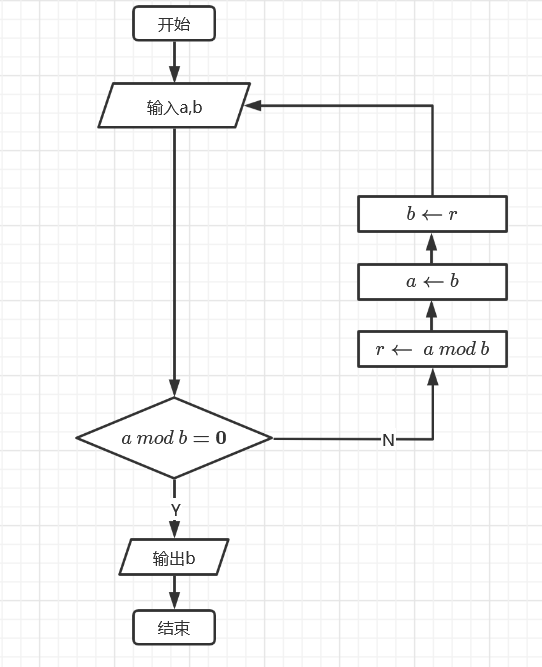
\includegraphics[scale=0.6]{一般欧几里得算法.png}} 
	\par 相关计算公式$gcd(a,b) = gcd(b,a\; mod\; b)$。
	\par 朴素欧几里得算法相关代码
	\begin{lstlisting}[ language=Java]
		public static int gcd(int a,int b){
		    while(b!=0){
		        int t=a%b;
		        a=b;
		        b=t;
		    }
		    return a;
		}
	\end{lstlisting}



\subsection{欧拉函数}
	\par 定义:一组数$x_1,x_2,...,x_n$称为模$m$的缩系,如果对$\forall j,s\in \mathbb{Z}, 1\leqslant j\leqslant s ,gcd(x_j,r)=1$,并定义$\phi(m)=s$,即${1,2,...,m}$中与$m$互质的数的个数,$\phi(m)$称为欧拉函数。
	\par 显然$\phi(1)=1$,而对于$m>1$,$\phi(m)$就是$1,2,...,m-1$中与m互质的数的个数。特别的,对于$p\in \{$素数$\}$,有$\phi(p)=p-1$。

\subsection{裴蜀定理}
	\par 定理:已知整数$a,b$和$d=gcd(a,b)$。若$a,b$是整数,那么对任意整数$x,y$,$ax+by$ 都一定是$d$的倍数,特别的,一定存在整数$x,y$,使$ax+by=d=gcd(a,b)$成立。
	\par 推论:$a,b$互质的充分必要条件是存在整数$x,y$,使$ax+by=1$。

\subsection{乘法逆元}
	\par 背景:已知整数$a,b$。现要根据$ax\equiv1\; mod \; b$ 计算x。
	\par 对于这个同余式,可以转换为$ax+by=1,(y\in \mathbb{Z})$,这个形式恰好符合裴蜀定理的形式,于是$gcd(a,b)=1$。这表明 $a,b$互质是逆元存在的必要条件。同理可以证明:$a,b$互质是 $a$在模 $b$ 下存在逆元的充分条件。

\subsection{费马小定理}
	\par 定理\upcite{1}:已知$p$为素数,$a$为任意自然数,则$a^{p}\equiv a\;(mod\; p)$。进一步,若$gcd(a,p)=1$,则$p|(a^{p-1}-1)$,即$a^{p-1}\equiv 1\; (mod \; p)$。
	\par 引理(二次探测定理)  如果$p$是一个素数,且$0<x<p$,则方程$x^2\equiv1 \; (mod\; p)$的解为$x=1 \; or \; p-1$。



\section{RSA算法过程}

\subsection{算法概述}
	\par 整个加密过程需要用到的参数如下

		\begin{table}[H] \wuhao             %局部字体设置大小
		   \centering
		  \caption{RSA算法相关符号}\label{tab}
		  \begin{tabular}{c|c}
		    \toprule                  %设置为顶线默认格式 加粗
		    符号 & 说明 \\
		    \hline                  %普通横线
		    ${{p}\mbox{、}{q}}$ & 两个随机素数 \\
		    $n$ & p和q的乘积 \\
		    $l$ & n的欧拉数 \\
		    $e$ & $(1,l)$区间内和$l$互质的随机整数 \\
			$d$ & $e$在模$l$下的乘法逆元\\
		\bottomrule                %设置为底线默认格式
		  \end{tabular}
		\end{table}

	\par 接收方生产私钥和公钥的基本过程如下: 
	\par 1、随机生成两个大素数$p、q$
	\par 2、令$n=p*q$
	\par 3、令$l=\phi(n)=(p-1)*(q-1)$
	\par 4、随机生成一个数$e$,满足$1<e<l$  且 $e$和$l$互质
	\par 5、由乘法逆元的原理,通过$(d*e)\space mod\space l=1$计算得到$d$
	\par 6、$(e,n)$作为公钥,$(d,n)$作为私钥

	\par 整体流程\upcite{2}如图:\\
	\centerline{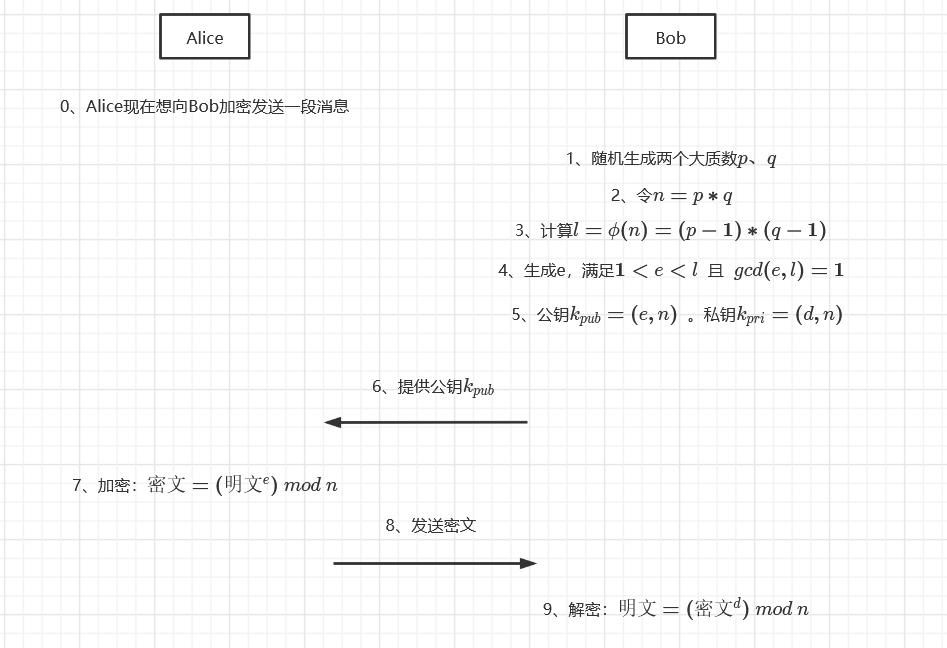
\includegraphics[scale=0.6]{RSA流程.png}} 


\subsection{辅助算法实现}

\subsubsection {扩展欧几里得算法与乘法逆元}
\paragraph{递推形式扩展欧几里得算法推导}
	\indent \;
	\par 欧几里得算法的另一个用途就是求解$(a,b)=ax+by$中的$x,y$。在欧几里得算法中,递归部分的核心等式为$gcd(a,b)=gcd(b,a\; mod \; b)=gcd(b,a-b\lfloor \dfrac{a}{b}\rfloor)$ ,由此式可以得出和$x,y$相关的递归关系。根据裴蜀定理,可以找到四个整数$x,y,x^{\prime},y^{\prime}$,使得\\
	$$
		\left\{
			\begin{array}{lr}
			ax+by=gcd(a,b)\\
			bx^{\prime}+(a-b\lfloor\dfrac{a}{b}\rfloor)y^{\prime}=gcd(b,a-b\lfloor\dfrac{a}{b}\rfloor)
			\end{array}
		\right.
	$$
	\par 由于等式右侧相等,所以有$ax+by=bx^{\prime}+(a-b\lfloor\dfrac{a}{b}\rfloor)y^{\prime}$,整理得到$a(x-y^{\prime})+b(y-(x^{\prime}-\lfloor\dfrac{a}{b}\rfloor y^{\prime}))=0$,因为$a,b$均不为0,所以有\\
	$$
		\left\{
			\begin{array}{lr}
			x-y^{\prime}=0\\
			y-(x^{\prime}-\lfloor\dfrac{a}{b}\rfloor y^{\prime})=0
			\end{array}
		\right.
	$$
	\par 即\\

	$$
		\left\{
			\begin{array}{lr}
			x=y^{\prime}\\
			y=x^{\prime}-\lfloor\dfrac{a}{b}\rfloor y^{\prime}
			\end{array}
		\right.
	$$

	\par 因此,要求解$x,y$,只需要递归求解更小规模的$x^{\prime},y^{\prime}$即可。计算到最后的边界条件$b=0$时,有$x=1,y=0$。


	\indent \;
	\par 在数据足够大时,采用递归方式的空间复杂度会急剧增加。现考虑将扩展欧几里得算法转化为递推形式以降低空间复杂度。
	\par 对于先前已知的递归式\\
	$$
		\left\{
			\begin{array}{lr}
			x=y^{\prime}\\
			y=x^{\prime}-\lfloor\dfrac{a}{b}\rfloor y^{\prime}
			\end{array}
		\right.
	$$
	\par 可以转换为矩阵形式\\
	$$
		\left(\begin{matrix}
		x\\
		y
		\end{matrix}\right)
		=
		\left(\begin{matrix}
		0 & 1\\
		1 & -d_{1}
		\end{matrix}\right)
		\left(\begin{matrix}
		x^{\prime}\\
		y^{\prime}
		\end{matrix}\right),
		\space (d_{1}=\lfloor\dfrac{a}{b}\rfloor)
	$$
	\par $x^{\prime},y^{\prime}$同样可以展开成上述形式,由此一直递推到$x=1,y=0$,形成下式\\

	$$  
		\left(\begin{matrix}x\\y\end{matrix}\right)
		=
		\left(\begin{matrix}0 & 1\\1 & -d_{1}\end{matrix}\right)
		\left(\begin{matrix}0 & 1\\1 & -d_{2}\end{matrix}\right)
		\left(\begin{matrix}0 & 1\\1 & -d_{3}\end{matrix}\right)
		...
		\left(\begin{matrix}0 & 1\\1 & -d_{n}\end{matrix}\right)
		\left(\begin{matrix}1\\0\end{matrix}\right)
	$$


	\par 每次迭代时,都可以从左向右计算一个矩阵,从而达到了迭代的目的。
	\par 假设在某次迭代之前计算的矩阵之积为$\left(\begin{matrix}m_{1} & m_{2}\\n_{1} & n_{2}\end{matrix}\right)$(迭代开始之前是一个单位阵),下一个待右乘的矩阵为$\left(\begin{matrix}0 & 1\\1 & -d_{t}\end{matrix}\right)$,二者之积可以写成\\
	$$
		\left(\begin{matrix}m_{1} & m_{2}\\n_{1} & n_{2}\end{matrix}\right)
		\left(\begin{matrix}0 & 1\\1 & -d_{t}\end{matrix}\right)
		=
		\left(\begin{matrix}m_{2} & m_{1}-d_{t}m_{2}\\n_{2} & n_{1}-d_{t}n_{2}\end{matrix}\right)
	$$
	\par 所有矩阵计算完成之后,得到一个最终矩阵$\left(\begin{matrix}M_{1} & M_{2}\\N_{1} & N_{2}\end{matrix}\right)$,这个矩阵满足$\left(\begin{matrix}x\\ y \end{matrix}\right) =\left(\begin{matrix}M_{1} & M_{2}\\N_{1} & N_{2}\end{matrix}\right) \left(\begin{matrix} 1 \\0\end{matrix}\right)$,展开可得$x=M_{1},y=N_{1}$。\\ \\
	
	\par 综上,递推的算法步骤如下:
	\par 1、给矩阵赋初值$\left(\begin{matrix}x & m\\y & n\end{matrix}\right) =\left(\begin{matrix}1 & 0\\0 & 1\end{matrix}\right) $ 

	\par 2、每次迭代时,计算$d=\lfloor\dfrac{a}{b}\rfloor$

	\par 3、更新矩阵
	   $$
	   \left(\begin{matrix}x & m\\y & n\end{matrix}\right) \leftarrow
	   \left(\begin{matrix}x & m\\y & n\end{matrix}\right) \left(\begin{matrix}0 & 1\\1 & -d\end{matrix}\right) =
	   \left(\begin{matrix}m & x-dm\\n & y-dn\end{matrix}\right)
	   $$

	\par 4、进行一般欧几里得算法的迭代
	   $$
	   \left(\begin{matrix}a\\b\end{matrix}\right) \leftarrow
	   \left(\begin{matrix}b\\a\space mod \space b\end{matrix}\right)
	   $$

	\par 5、$b=0$时,计算结束,此时已经求出需要的$x,y$,并且最大公约数存如变量$a$中。
	\par 递推代码如下
	\begin{lstlisting}[ language=Java]
		//java无法传入指针,这里array[0]代表x,array[1]代表y
		public static long exgcd(long a,long b,long[] array){
		    long m=0;
		    long n=1;
		    while(b>0){
		        long d=a/b;
		        long t;
		        
		        t=m; m=array[0]-d*t; array[0]=t;
		        t=n; n=array[1]-d*t; array[1]=t;
		        t=a%b; a=b; b=t;
		    }
		    return a;
		}
	\end{lstlisting}
	
	\par 下面为采用BigInteger的代码形式(由于可读性相对低,本文只在此处展示BigInteger相关代码)
	\begin{lstlisting}[ language=Java]
		public static BigInteger exgcd(BigInteger a,BigInteger b,BigInteger[] array){
		    BigInteger m=new BigInteger("0");
		    BigInteger n=new BigInteger("1");
			while(b.compareTo(zero)>0){
		        BigInteger d=a.divide(b); 
		        BigInteger t;
		
		        t=m; m=array[0].add(d.negate().multiply(t)); array[0]=t;
		        t=n; n=array[1].add(d.negate().multiply(t)); array[1]=t;
		        t=a.mod(b); a=b; b=t;
		    }
		    return a;
		}
	\end{lstlisting}



\paragraph{乘法逆元计算}
	\indent \;
	\par 当使用扩展欧几里得算法找到一组$x,y$ 满足$ax+by=1$时,就可以得出$ax\equiv 1\; (mod\; b)$,即$x$是$a$的乘法逆元,那么对$\forall x+kb,k\in \mathbb{N}$也都是$a$的乘法逆元,这表明,一定有$a$的一个乘法逆元在区间 $[0,b)$ 内。
	\par 利用前面完成的扩展欧几里得算法,找到$n$在模$p$下的乘法逆元。代码如下
	\begin{lstlisting}[ language=Java]
		public static long inv(long a,long p){
	    	long[] array={1,0}; //array[0]代表x,array[1]代表y
	    	if(exgcd(a,p,array)==1){
	        	array[0]%=p;
	        	return array[0]>=0 ? array[0]:array[0]+p;
	    	}
	   		else return -1;  //-1代表不存在对应的乘法逆元
		}
	\end{lstlisting}

\subsubsection{快速模幂运算}
	\par 快速模幂算法基于快速幂多了一些取模运算,整体思想相同。快速幂的核心思想是每一步都将指数减半,相应的底数做平方运算,这样可以达到快速降低指数的目的。
	\par 例如:已知$a,b$求$a^{b}$,假设$b=11$。
	\par 这里可以将表达式的指数写成二进制的形式
	$$
		a^{11}=a^{2^{3}+2^{1}+2^{0}}=a^{(1011)_{2}}
	$$

	\par 指数减半等价于对指数的二进制形式右移一位,假如当前末位为0,则直接进行移位运算。若当前末尾不为0,则提出一个当前底数后,再将指数右移一位。如$a^{(1011)_{2}}=a*a^{(1010)_{2}}=a*(a^{2})^{(101)_{2}}$

	\par 相关代码如下
	\begin{lstlisting}[ language=Java]
		public static long qmod(long a,long p,long mod){
		    long ans=1;
		    a%=mod;
		    while(p>0){
		        if((p&1)==1){  //p为奇数,则需要拿出一个a,指数减一成为偶数后,再将指数右移一位
		            ans=(ans*a)%mod;  //ans在整个计算过程中都会比mod小,不需要额外进行取模操作
		        }
		        a=(a*a)%mod;
		        p>>=1;  //p右移一位
		    }
		    return ans;
		}
	\end{lstlisting}
	
\subsubsection{大素数判定}

\paragraph{费马素性测试}
	\indent \;
	\par 该测试基于费马小定理。费马小定理对所有素数都成立,因此,对于一个待测数$p$,可以随机挑选$[2,p-2]$中的任一整数$t$,若存在$t$不满足$a^{t-1}\equiv 1 \;(mod \; p)$,说明$p$不是素数。测试次数越大,则素数判定的正确性越高。

	\par 但是某些合数也满足费马小定理,这样的合数称为卡迈克尔数。给定卡迈克尔数$C$,对所有满足$gcd(a,C)=1$的整数$a$,都满足$a^{C-1}\equiv 1\; (mod\; C)$。$n=561=3*11*17$就是一个卡迈克尔数。

\paragraph{Miller-Rabin算法测试}
	\indent \;
	\par 费马素性测试的测试范围不够大,实践中更多会采用Miller-Rabin算法进行测试\upcite{4}。
	\par 假设$n$是奇素数,则$n-1$必为偶数,令$n-1=2^q*m$。
	\par 随机选取整数$a(1<a<n)$,由费马小定理知$(a^{2^{q}*m}=a^{n-1})\equiv1\; (mod \; n)$ 。
	\par 由二次探测定理知:$a^{2^{q-1}*m}\equiv 1\; (mod\; n)\;$或$\; a^{2^{q-1}*m}\equiv n-1\; (mod\; n)$。
	\par 若$a^{2^{q-1}*m}\equiv 1\; (mod\; n)$ 成立,则再由二次探测定理可知:$a^{2^{q-2}*m}\equiv 1\; (mod\; n)\;$或$\; a^{2^{q-2}*m}\equiv n-1\; (mod\; n)$。
	\par 如此反复,直到某一步$a^{m}\equiv 1\; (mod \; n)\;$ 或$\; a^{m}\equiv n-1\; (mod \; n)$ 。如果$n$是素数,则$a^m\equiv 1\; (mod \; n)\;$ ,或存在$\; 0\leq r\leq q-1 \;$ 使 $\; a^{2^{r}*m}\equiv 1\; (mod\; n)$。 \\
	\indent \;
	\par 算法思路为:
	\par 1、给定奇数n,为了判定n是不是素数,首先测试$a^{2^{q}*m}\equiv1\space (mod \space n)$,是否成立(这一步需要使用快速模幂算法),若不成立,则n一定是合数;若成立,则继续运行算法。
	\par 2、考察下面的Miller序列:
	$$
		a^{2^{0}m}(mod\space n),a^{2^{1}m}(mod\space n),a^{2^{2}m}(mod\space n),...a^{2^{q-1}m}(mod\space n),
	$$
	\par 若$a^{m}\equiv 1\space(mod \space n)$,或存在$0\leq r\leq q-1$ 使 $a^{2^{r}m}\equiv 1\space (mod\space n)$ 成立,则通过测试。 \\
	
	\par 相关代码如下
	\begin{lstlisting}[ language=Java]
		public static boolean millerRabin(long num){
    		if(num==2) return true;
    		else if(num<2 || (num&1)==0) return false;

    		int judgeTime=100;  //随机挑100个数进行判定,可以定义判断的次数
		    long m=num-1;
		    long t=0;
		    //计算 num-1=m*(2^t) 的m和t
		    while((m&1)==0) {
		        m >>= 1;
		        t++;
		    }

		    for(int i=1;i<=judgeTime;i++){
		        //[2,num-1]中的随机数a
		        long a=(long)(Math.random()*(num-2)%num+2);
		        //计算 a^m % num
		        long x=qmod(a,m,num),y=x;
		
		        for(int j=0;j<t;j++){
		            y=qmod(x,2,num); //x^2 mod num
		            //不满足二次探测定理,也就是y==1了但是x并不等于1或者n-1,那么n就一定不是素数
		            if(y==1 && x!=1 && x!=num-1){
		                return false;
		            }
		            x=y;
		        }
		        //子循环结束后,y仍不为1,则num不是素数
		        if(x!=1) return false;
		    }
		    return true;
		}
	\end{lstlisting}


\section{总结}
	\par RSA是目前使用广泛的一种公钥密码系统,它的安全性基于大整数因子分解难题\upcite{5}。目前主流的电子计算机的算力尚不能快速破解经RSA加密的密钥,同时,RSA生成的密钥长度从以前的1024位发展到了现在的2048位和3082位,因此目前RSA加密的安全性还是有所保证的。RSA 密码系统可用于消息加密和数字签名,密码强度主要与RSA模数N的长度有关,目前长度是2048位,即256字节,非常安全。经过本次RSA算法的粗略设计与实现,一定程度上能够提高对数论与编程的认知,这对今后了解更前沿的密码算法大有裨益。

\begin{thebibliography}{5}
	\bibitem{1}费马小定理 https://zhuanlan.zhihu.com/p/87611586
	\bibitem{2}RSA算法分析 https://zhuanlan.zhihu.com/p/36347853
	\bibitem{3}扩展欧几里得算法 https://zhuanlan.zhihu.com/p/58241990
	\bibitem{4}Miller-Rabin素性测试 https://blog.csdn.net/ECNU\_LZJ/article/details/72675595
	\bibitem{5}王生玉,汪金苗,董清风,等.基于属性加密技术研究综述[J].信息网络安全,2019,19(9):76-80
\end{thebibliography}

 
\end{document}